\chapter{Fault Modeling and the Safety Annex}
\label{chap:faultModeling}
Early on in Section~\ref{subsec:mbsa}, a model-based safety assessment process was proposed. This process was backed by formal methods and incorporates a shared model into the development and safety analysis processes. A high level description of this cyclical process is shown in Figure~\ref{fig:SACycle} for your convenience. 

\begin{figure}[h]
	\begin{center}
		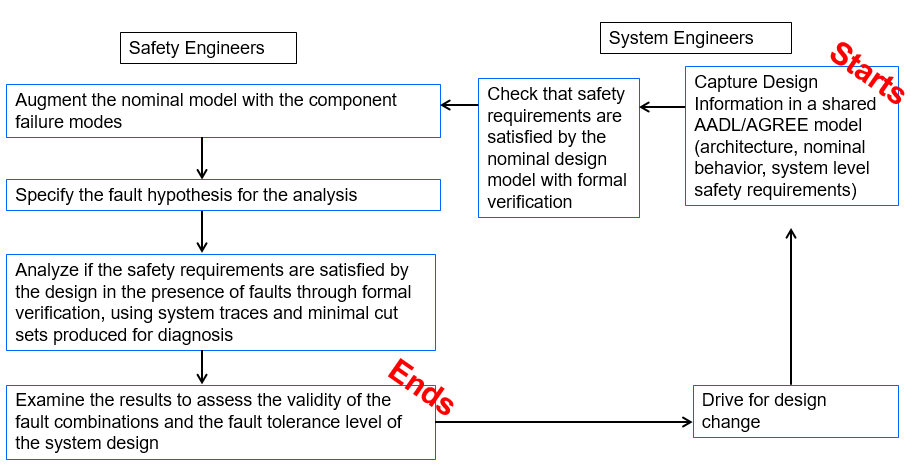
\includegraphics[width=\textwidth]{images/process4.PNG}
	\end{center}
	\caption{Proposed Steps of the Safety Assessment Process}
	\label{fig:SACycle}
\end{figure}

There are certain capabilities that are required in order to fully perform all steps of this process. In beginning this research, we outlined what those pieces were and investigated related work to determine if a gap still existed. Based on the related work summary found in Section~\ref{sec:modelCheckingInSA}, it can be seen that this research attempts to fill certain gaps in the field of safety analysis. 

\begin{description}[nosep]

    \item[Shared model] with a language expressive enough to describe HW and SW components.
    \item[Flexible error propagations] through both behavioral and explicit means.
    \item[Flexible fault modeling] with support for a/symmetric faults, in/dependent faults, etc.
    \item[Model checker] used to assess and verify the design with or without faults active.
    \item[Ability to generate artifacts] used in the safety assessment process.
\end{description}

In this chapter, the fault modeling process using the Safety Annex for the Architecture Analysis and Design Language (AADL)~\cite{AADL_Standard} is described. The Safety Annex was developed with these two broad ideas in mind: (1) how the safety annex can support the proposed safety assessment process, and (2) what are the gaps in current related safety analysis tools that can be closed with this research.

\section{Fault, Failure, and Error Terminology}
The usage of the terms error, failure, and fault are defined in ARP4754A and are described here for ease of understanding~\cite{SAE:ARP4754A}. An \textit{error} is a mistake made in implementation, design, or requirements. A \textit{fault} is the manifestation of an error and a \textit{failure} is an event that occurs when the delivered service of a system deviates from correct behavior. If a fault is activated under the right circumstances, that fault can lead to a failure. The terminology used in the Error Model Annex version 2 for AADL (EMV2)~\cite{EMV2}, differs slightly for an error: an error is a corrupted state caused by a fault. The error propagates through a system and can manifest as a failure. In this dissertation, we use the ARP4754A terminology with the added definition of \textit{error propagation} as used in EMV2. An error is a mistake made in design or code and an error propagation is the propagation of the corrupted state caused by an active fault. 

\section{Implementation of the Safety Annex}
\label{sec:impl}
%Important features were considered before the implementation of the safety annex; these we addressed one by one and will outline below. 

As described in Section~\ref{sec:concepts}, an AADL~\cite{AADL_Standard} model describes a system in terms of a hierarchy of components and their interconnections, where each component can either represent a logical entity (e.g., application software functions, data) or a physical entity (e.g., buses, processors). AADL is used to specify and analyze real-time embedded systems. It includes specifications specific to hardware, software, and system component abstractions. The language definition is sufficiently rigorous to support formal analysis tools that allow for early phase error/fault detection~\cite{FeilerModelBasedEngineering2012}. 

\begin{figure}[h!]
	%\vspace{-0.1in}
	\begin{center}
	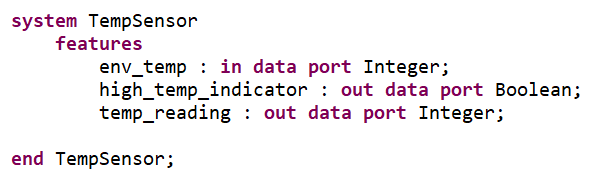
\includegraphics[width=.8\textwidth]{images/aadlComponent.png}
	\caption{AADL Component Types}
	\label{fig:aadlComponent}
	%\vspace{-0.2in}
	%\vspace{-0.1in}
	\end{center}
\end{figure}

Central to an AADL model are component \emph{types} and \emph{implementation} declarations. Figure~\ref{fig:aadlComponent} shows an example of a simple sensor component type defined in AADL. The component has an environmental temperature as input and two outputs: a high temperature indication and a temperature reading. In the type declaration, you define the category (\texttt{system} in this example) and features such as inputs and outputs; the implementation contains definitions of the internal structure of the component, e.g., internal constituents and their interactions. 

\begin{figure}[h!]
	%\vspace{-0.1in}
	\begin{center}
	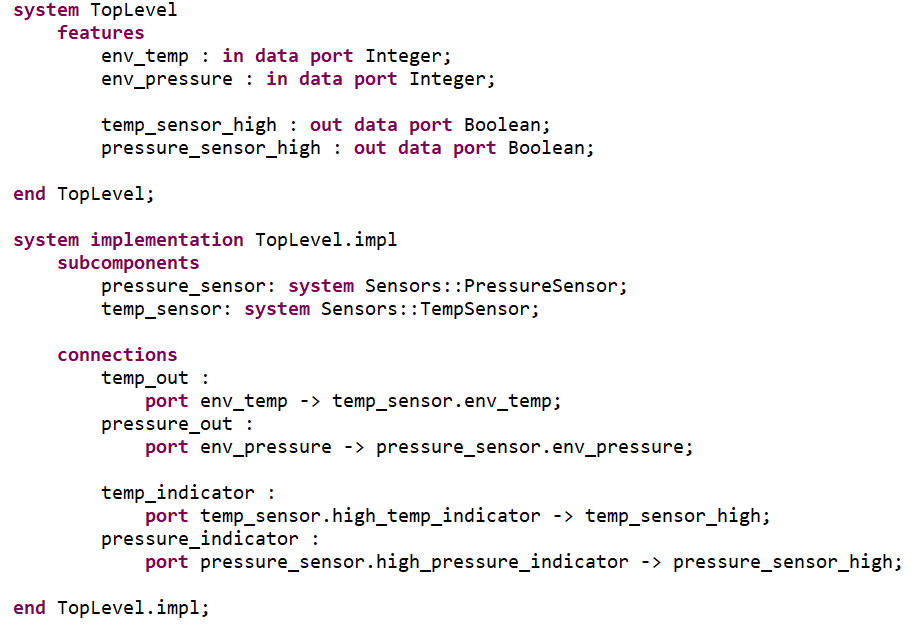
\includegraphics[width=1.0\textwidth]{images/aadlImplementation.png}
	\caption{An AADL Component Implementation Definition}
	\label{fig:aadlImplementation}
	%\vspace{-0.2in}
	%\vspace{-0.1in}
	\end{center}
\end{figure}

An implementation of the sensor component type is shown in Figure~\ref{fig:aadlImplementation}. The system contains a type of its own (top of figure: \texttt{system TopLevel}) which holds any environmental inputs or subcomponent outputs. The implementation defines the subcomponents of the system and their connections (bottom half of figure). 

Since AADL supports model-based system development and the language definition is sufficiently rigorous to support formal analysis tools that allow for early phase error/fault detection~\cite{FeilerModelBasedEngineering2012}, this language was chosen for this research. 

As described in Section~\ref{subsec:mbsa}, {\em nominal model analysis} is a part of the MBSA process. The nominal model consists of the system model architectural design as well as behavioral contracts for each component and requirement specifications. The verification at the nominal level consists of showing that the model satisfies the specified requirements in the absence of faults. 

The Assume-Guarantee Reasoning Environment (AGREE)~\cite{cofer2012compositional} is a language annex for AADL that provides a mechanism for the specification of component requirements in formal logic and utilizes a model checker to provide proofs regarding these specifications as described in Section~\ref{sec:concepts}. 

\begin{figure}[h!]
	%\vspace{-0.1in}
	\begin{center}
	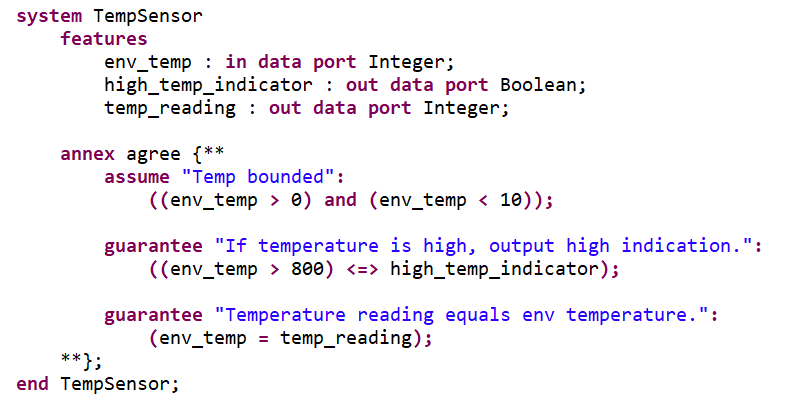
\includegraphics[width=1.0\textwidth]{images/agreeContract2.png}
	\caption{The AGREE Contract for an AADL Component Type}
	\label{fig:agreeContract}
	%\vspace{-0.2in}
	%\vspace{-0.1in}
	\end{center}
\end{figure}

An example of an AGREE contract is shown in Figure~\ref{fig:agreeContract} and is placed in the context of the AADL temperature sensor component shown in Figure~\ref{fig:aadlComponent}.  An AGREE contract consists of {\em assumptions} on the inputs of AADL components that constrain what the component sees from the environment and {\em guarantees} on the outputs that constrain how the component behaves given its environment. In this example, the assumption restricts the environmental temperature to be within a range of values; the guarantee defines the behavior of the component given the environment. 

Since our desire was to facilitate {\em behavioral error propagation}, AGREE was a suitable and obvious choice for the nominal verification tooling. 

Through AGREE, the nominal model is translated into the dataflow programming language Lustre~\cite{Halbwachs91:IEEE} that is used as input to the JKind model checker~\cite{2017arXiv171201222G}. JKind uses a series of backend SMT-solvers to generate proofs of the top level AGREE properties specified in the model. When there exists a trace such that a property is invalid, JKind provides a {\em counterexample} showing the system trace in which the property is violated. An example of this is shown in Figure~\ref{fig:coex}. 

\begin{figure}[h!]
	%\vspace{-0.1in}
	\begin{center}
	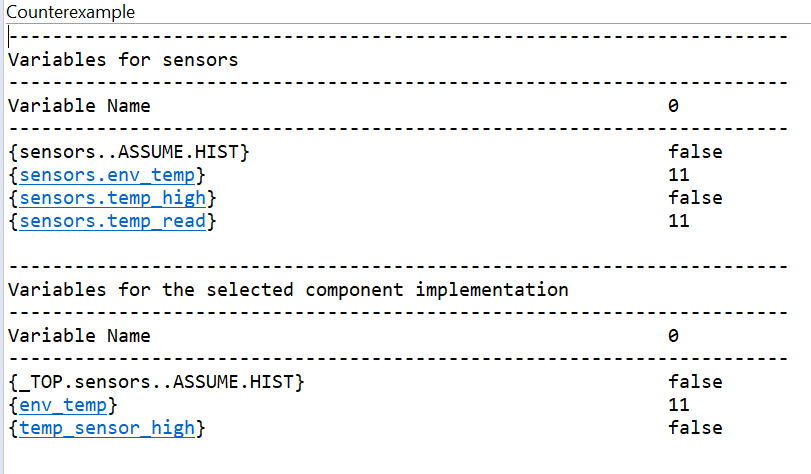
\includegraphics[width=1.0\textwidth]{images/coex.png}
	\caption{A Counterexample to an Invalid Property}
	\label{fig:coex}
	%\vspace{-0.2in}
	%\vspace{-0.1in}
	\end{center}
\end{figure}

The model checker takes an adversarial role in the proof process by trying to find paths such that the proof is violated. If none exist, then the results are valid. This adversarial role is exactly what we wished to harness for this kind of analysis. If we allow faults to be active, but leave them unconstrained, this allows the model checker to determine if certain faults could lead to a violation of a property. These counterexamples could then contain fault information. 

Given that AGREE guarantees define the {\em output} behavior of components, any connected component's assumptions rely on those guarantees. If an assumption is violated, the guarantee may not hold. By associating a fault with the output of a component, this fault -- when active -- may violate assumptions and guarantees along the signal flow within a system. This was our goal; we wished to view the behavioral propagation of an active fault. 

\subsection{Implementation Architecture}
\label{sec:implArchitecture}
The safety annex is written in Java as a plug-in for the OSATE AADL toolset, which is built on Eclipse.  It is not designed as a stand-alone extension of the language, but works with behavioral contracts specified using the AGREE annex for AADL~\cite{NFM2012:CoGaMiWhLaLu}. 
The architecture of the Safety Annex is shown in Figure~\ref{fig:plugin-arch}.

\begin{figure}[h]
	\begin{center}
		%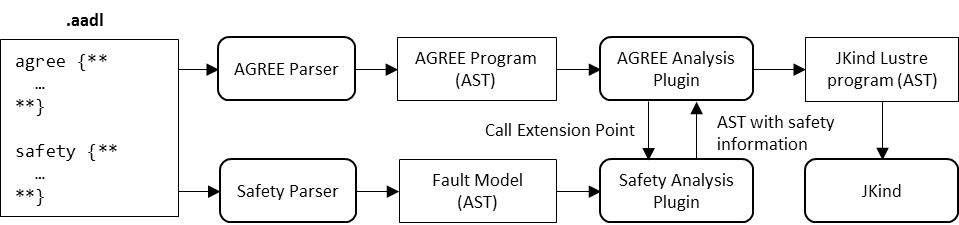
\includegraphics[trim=0 400 430 0,clip,width=0.85\textwidth]{images/arch.png}
		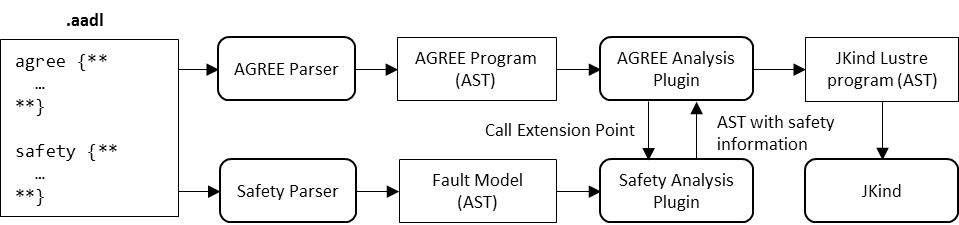
\includegraphics[width=\textwidth]{images/arch.png}
	\end{center}
	%\vspace{-0.2in}
	\caption{Safety Annex Plug-in Architecture}
	\label{fig:plugin-arch}
	%\vspace{-0.2in}
\end{figure}

The safety language extension resides in an annex of AADL and the faults defined therein are translated into an abstract syntax tree and inserted into the AGREE program. The AGREE program contains the building blocks for the translation into Lustre which is the program directly analyzed by JKind.  

When performing fault analysis, the fault definitions defined in the safety annex extend the AGREE contracts to allow faults to modify the behavior of component outputs. The temperature sensor subcomponent shown in Figure~\ref{fig:agreeContract} encoded into Lustre is shown in Figure~\ref{fig:lustreTempNode}\footnote{The Lustre code is slightly simplified for readability.}.

\begin{figure}[h]
	\begin{center}
		%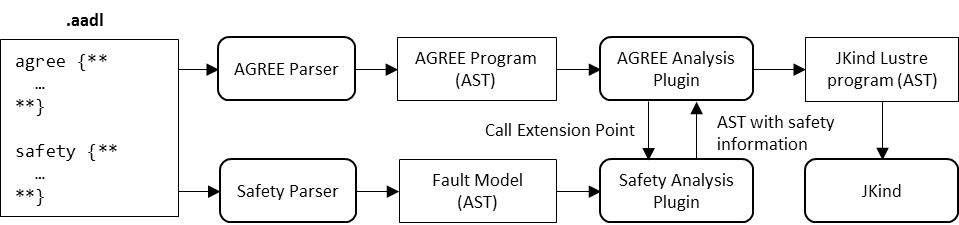
\includegraphics[trim=0 400 430 0,clip,width=0.85\textwidth]{images/arch.png}
		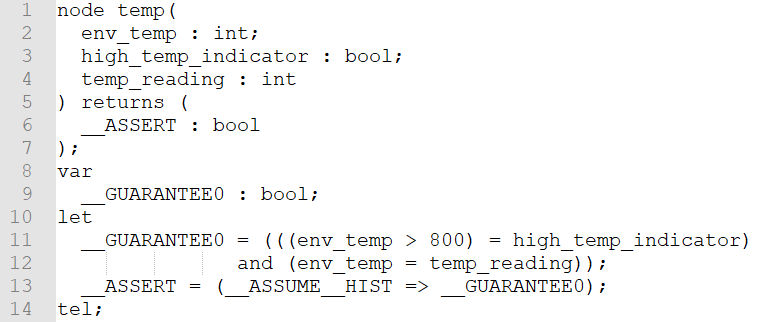
\includegraphics[width=0.8\textwidth]{images/lustreTempNode.png}
	\end{center}
	%\vspace{-0.2in}
	\caption{Temperature Component in Lustre}
	\label{fig:lustreTempNode}
	%\vspace{-0.2in}
\end{figure}

The inputs and outputs (lines 2-4) correspond directly to the AADL inputs and outputs of the component; likewise, the guarantee (\texttt{\_\_GUARANTEE0}) corresponds to the guarantee on the outputs. The \texttt{\_\_ASSERT} statement on line 13 states that as long as the assumptions hold, the guarantee is implied. 

From the perspective of fault analysis, we want to insert a fault on the output of the component. This fault may or may not be active -- it is up to the model checker. To this end, we specify three variables per potentially faulty output: \texttt{fault\_nominal}, \texttt{fault\_trigger}, and \texttt{fail\_val}. If the trigger is true, then output failure value, else output nominal value. This can be seen in Figure~\ref{fig:lustreTempNodeFault}: the new variables are assigned as inputs (lines 4-6) and the assert statement in line 20 shows the triggering behavior.

\begin{figure}[h]
	\begin{center}
		%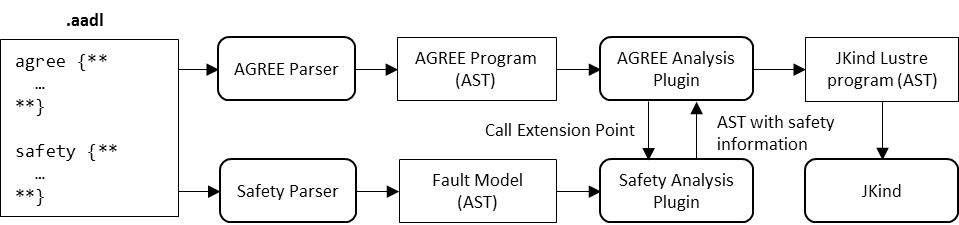
\includegraphics[trim=0 400 430 0,clip,width=0.85\textwidth]{images/arch.png}
		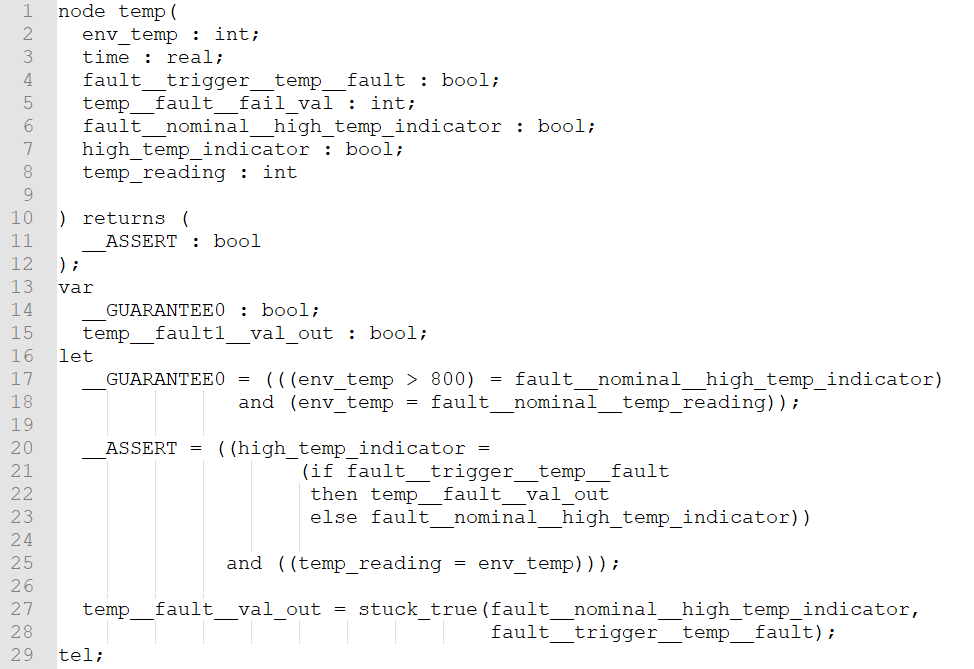
\includegraphics[width=0.8\textwidth]{images/lustreTempNodeFault.png}
	\end{center}
	%\vspace{-0.2in}
	\caption{Temperature Component with Fault in Lustre}
	\label{fig:lustreTempNodeFault}
	%\vspace{-0.2in}
\end{figure}

This allows for the possibility of active faults, but when the faults are inactive, the nominal value is simply passed through. Line 27 of Figure~\ref{fig:lustreTempNodeFault} shows a call to what we call a {\em fault node}; this is the code that specifies the behavior of an active fault. The fault node \texttt{stuck\_true} is shown in Figure~\ref{fig:lustreFaultNode}. The behavior of an active fault is to output {\em true}. The \texttt{trigger} input to the fault node corresponds directly with the trigger defined in the temperature node of Figure~\ref{fig:lustreTempNodeFault} on line 4. 

\begin{figure}[h]
	\begin{center}
		%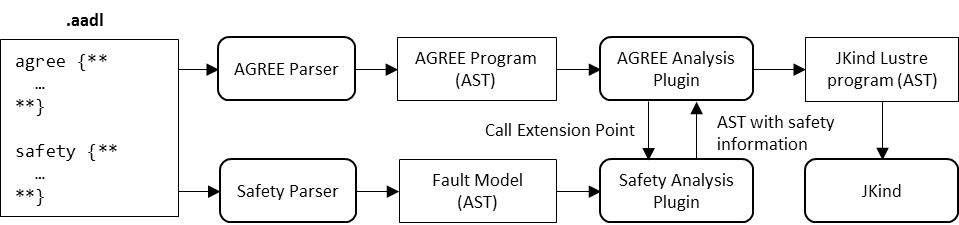
\includegraphics[trim=0 400 430 0,clip,width=0.85\textwidth]{images/arch.png}
		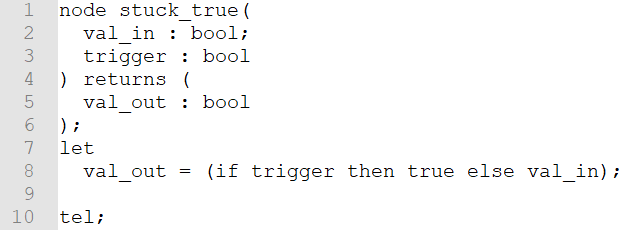
\includegraphics[width=0.8\textwidth]{images/lustreFaultNode.png}
	\end{center}
	%\vspace{-0.2in}
	\caption{A Fault Node in Lustre}
	\label{fig:lustreFaultNode}
	%\vspace{-0.2in}
\end{figure}
 
The model elements are translated into Lustre formulae. These are represented in JKind as a transition system, and reasoning is performed using $k$-induction. At each time-step of analysis, every formula in the model is given an assignment based on the constraints over that formula. If every assignment results in a provable property over $k$ steps of induction, the property holds. When performing safety analysis over the model, each fault is defined as an {\em activation literal} and is unconstrained. If the assignment to an activation literal is {\em true}, this corresponds to an active fault and potentially violated guarantee. If that assignment violates a guarantee, then this violation will be reflected in the analysis results. At a system level, it can be seen if a violated guarantee will in turn violate the top level property. Hence it is seen how active faults at leaf level components violate the system level properties. 

This analysis approach allows for implicit propagation of violations throughout the system. It also allows for arbitrary temporal activations of faults. There are no explicit constraints put on faults stating when an activation can occur, which allows the model checking procedure free reign to activate the faults at the worst possible times. If there are dependencies regarding fault activations, these are handled through the use of explicit error propagations (see Section~\ref{sec:propogation}).

The main constraint put on the model checker in terms of the activation of faults consist of {\em fault hypothesis statements}. These constrain the model by stating either the number of faults that may be active at once, or the overall probability threshold that is allowed. In the latter case, each fault has an associated probability; assuming independence, the probability of a set of faults occurring should not be less than the threshold defined. 

There are two different types of fault analysis that can be performed on a fault model: verification in the presence of faults or the generation of minimal cut sets. The Safety Annex plugin intercepts the AGREE program and adds fault model information depending on which type of fault analysis is being run. For more information on types of fault analysis, see Section~\ref{sec:analysisResults}.










\section{Running Example: Sensor System}
\label{sec:sensorExample}
We present a running example of a simplified sensor system in a Pressurized Water Reactor (PWR). In a typical PWR, the core inside of the reactor vessel produces heat. Pressurized water in the primary coolant loop carries the heat to the steam generator. Within the steam generator, heat from the primary coolant loop vaporizes the water in a secondary loop, producing steam. The steamline directs the steam to the main turbine, causing it to turn the turbine generator, which produces electricity. There are a few important factors that must be considered during safety assessment and system design. An unsafe climb in temperature can cause high pressure and hence pipe rupture, and high levels of radiation could indicate a leak of primary coolant~\cite{PWR}. 

\begin{figure*}[h!]
	%\vspace{-2em}
	\begin{center}
		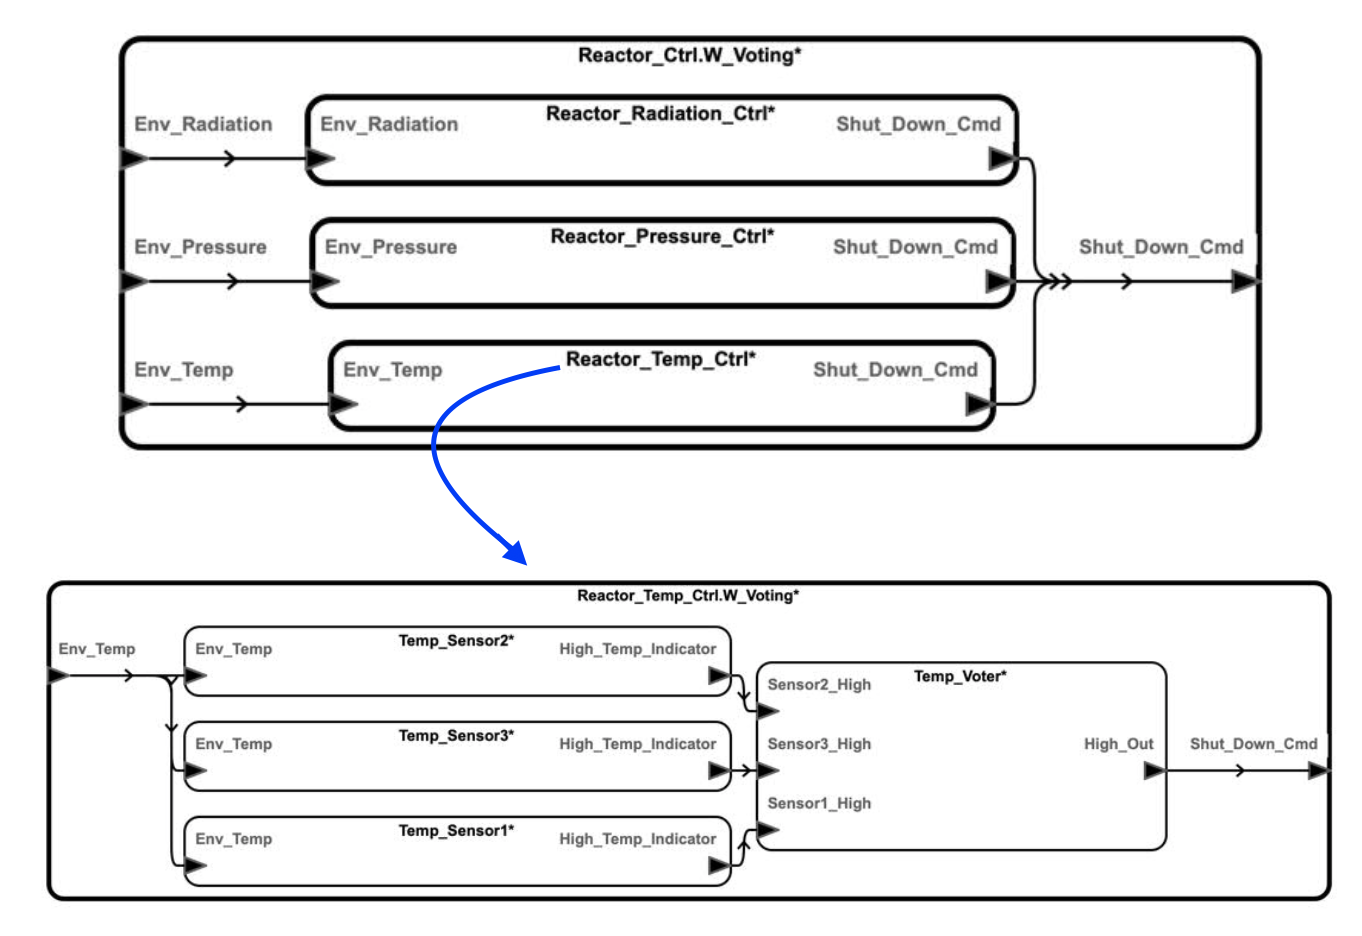
\includegraphics[width=0.6\textwidth]{images/sensorSysAADL.png}
	\end{center}
	\vspace{-2em}
	\caption{PWR Sensor System}
	\label{fig:sensorSys1}
	%\vspace{-2em}
\end{figure*}

The following sensor system can be thought of as a subsystem within a PWR that monitors these factors. A diagram of the model is shown in Figure~\ref{fig:sensorSys1} and represents a highly simplified version of a safety critical system. The temperature subsystem details are shown at the bottom of Figure~\ref{fig:sensorSys1}; each of the subsystems have a similar architecture.

The subsystems each contain three sensors that monitor pressure, temperature, and radiation. Environmental inputs are fed into each sensor in the model and the redundant sensors monitor temperature, pressure, or radiation respectively. If temperature, pressure, or radiation is too high, a shut down command is sent from the sensors to the parent components. 

\subsubsection{PWR Nominal Model}
The temperature, pressure, and radiation sensor subsystems use a majority voting mechanism on the sensor values and will send a shut down command based on this output. The safety property of interest in this system is: \emph{shut down when and only when temperature, pressure, or radiation is above the respective threshold}; the AGREE guarantee stating this property is shown in Figure~\ref{fig:shutdownGuar}. 

\begin{figure*}[h!]
	%\vspace{-2em}
	\begin{center}
		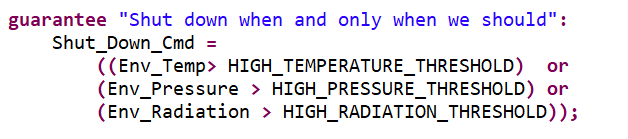
\includegraphics[width=0.6\textwidth]{images/sensorGuar.PNG}
	\end{center}
	\vspace{-2em}
	\caption{Sensor System Safety Property}
	\label{fig:shutdownGuar}
	%\vspace{-2em}
\end{figure*}

The safety of the system requires a shut down to take place if the temperature, pressure, or radiation levels climb beyond safe levels; thus, a threshold for each subsystem is introduced. If any sensor subsystem reports passing its threshold, a shutdown command is sent. Supporting guarantees are located in each sensor subsystem and correspond to temperature, pressure, and radiation sending a shut down command if sensed inputs are above a given threshold. Each sensor has a similar guarantee. 

Throughout the remainder of this chapter, we refer to the PWR example for illustrative purposes. The goal is to take the nominal system model and extend it to become a fault model using the safety annex. 

\section{Component Fault Modeling in the Safety Annex}
The safety annex is used to add possible faulty behaviors to a component model. When a fault is activated by its specified triggering conditions, it modifies the output of the component. This erroneous behavior may violate the contracts of other components in the system, including assumptions of downstream components. The impact of an active fault is computed by the AGREE model checker when the safety analysis is run on the fault model. 

When given a nominal model with which to perform safety analysis, the analyst must associate faults with each component. Examples of such faults include valves being stuck open or closed, output of a software component being nondeterministic, or power being cut off. These are often determined based on hardware specification guidelines and domain expertise. Returning to the PWR running example, each sensor for each subsystem may fail to indicate that the threshold has been surpassed. If the radiation levels are high and the radiation sensor reports no such indication, this is a fault that must be considered during analysis. 

As an illustration of fault modeling using the safety annex, we look at one of the components important to the PWR system level safety property: the radiation sensor.  If the radiation levels are high, the radiaton sensor reports this through an indicator to the radiation sensor subsystem. A shut down command will be sent to the top level. Figure~\ref{fig:radiationSensor} shows the AADL pedal sensor component with a contract for its nominal behavior. The sensor has only one input, the environmental radiation, and one output, the high radiation levels indication. The property that governs the behavior of the component is that the radiation sensor will indicate when the threshold is reached.

\begin{figure}[h!]
	%\hspace*{-2cm}
	%\vspace{-0.55in} 
	\begin{center}
		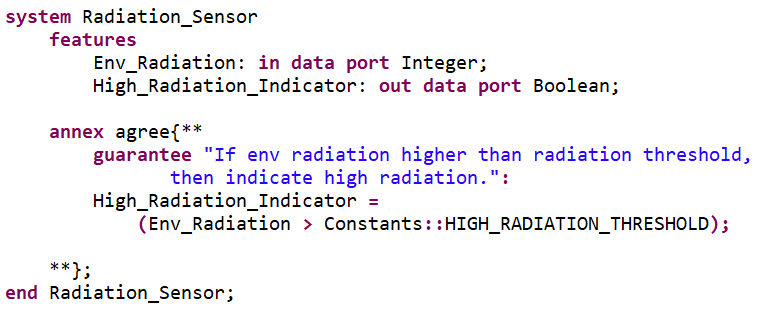
\includegraphics[width=0.8\textwidth]{images/radiationSensor.png}
		%\vspace{-0.3in}
		\caption{PWR Radiation Sensor}
		\label{fig:radiationSensor}
	\end{center}
	%\vspace{-0.2in}
\end{figure}

One possible failure for this sensor is inversion of its output value; the radiation levels are actually above threshold, but the sensor does not indicate such. This fault can be triggered with probability $1.0\times 10^{-5}$\footnote{In practice, the component failure probability is 
collected from hardware specification sheets.}. The safety annex definition for this fault is shown in Figure~\ref{fig:radiationSensorFault}. Fault behavior is defined through the use of a fault node called \textit{stuck\_false} (shown in Figure~\ref{fig:stuckFalseNode}).  When the fault is triggered, the nominal output of the component (\textit{High\_Radiation\_Indicator}) is replaced with its failure value (\textit{val\_out}). 

\begin{figure}[h!]
	%\hspace*{-2cm}
	%\vspace{-0.55in} 
	\begin{center}
		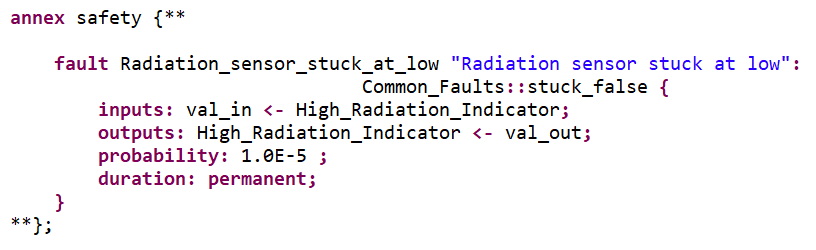
\includegraphics[width=0.8\textwidth]{images/radiationSensorFault.png}
		%\vspace{-0.3in}
		\caption{PWR Radiation Sensor Fault}
		\label{fig:radiationSensorFault}
	\end{center}
	%\vspace{-0.2in}
\end{figure}

Similar faults can be defined for all sensors in the PWR system. These may include stuck high (sensor reports high when threshold is not reached), stuck low (sensor does not report high when threshold is reached), etc. 
\begin{figure}[h!]
	\hspace*{-2cm}
	\vspace{-0.1in} 
	\begin{center}
		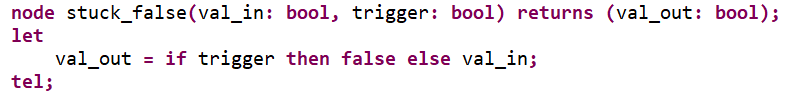
\includegraphics[scale=0.8]{images/stuckFalseNode.png}
	\caption{A Fault Node Definition}
		\label{fig:stuckFalseNode}
	\end{center}
\end{figure}

Given the complexity of systems, there are many types of faults that correspond to various components. The safety annex allows for complex fault behavior to be modeled through the node definitions and this can benefit safety analysts from numerous disciplines. The majority of faults that are connected to outputs of components are known as \textit{symmetric}. That is, whatever components receive this faulty output will receive the same faulty output value. Thus, this output is seen symmetrically. An alternative fault type is \textit{asymmetric}. This pertains to a component with a 1-n output: one output which is sent to many receiving components. For more information on modeling asymmetric faults, see Section~\ref{sec:byzantine}. %This fault can present itself differently to the receiving components. For instance, in a boolean setting, one component might see a true value and the rest may see false. This is also possible to model using the keyword \textit{asymmetric}. For more details on fault definitions and fault modeling capabilities, we refer readers to the Safety Annex Users Guide\cite{SAGithub}.



\section{Error Propagation}
As systems become larger and more complex, it can be difficult knowing all possible error propagations within a model; using a purely explicit approach to error propagation is difficult. To this end, we developed the Safety Annex to primarily use \textit{behavioral} propagation. In this approach, the faults are attached to a component's output and ``turned on" in a manner of speaking. The effects and propagation of the active fault is revealed through the behavioral contracts of the system by use of the model checker. 

This section outlines the Safety Annex approach to implicit error propagation and also describes how one can model an explicit propagation by defining dependent faults. 

\subsection{Implicit Propagation}
In the Safety Annex approach, faults are captured as faulty behaviors that augment the system behavioral model in AGREE contracts. No explicit error propagation is necessary since the faulty behavior itself propagates through the system just as in the nominal system model. The effects of any triggered fault are manifested through analysis of the AGREE contracts. In this way, the safety analysis is closely tied to the behavior model of components and their requirements; the analysis is focused on the system dynamics and interactions. 

In the PWR running example, all error propagations are defined implicitly. 

\begin{comment}
On the contrary, in the AADL Error Model Annex, Version 2 (EMV2)~\cite{EMV2} approach, all errors must be explicitly propagated through each component (by applying fault types on each of the output ports) in order for a component to have an impact on the rest of the system. To illustrate the key differences between implicit %failure
error propagation provided in the Safety Annex and the explicit %failure 
error propagation provided in EMV2, we use a simplified behavioral flow from the WBS example using code fragments from EMV2, AGREE, and the Safety Annex. 

\begin{figure}[h]
	%\hspace*{-2cm}
%	\vspace{-0.19in}
	\centering
	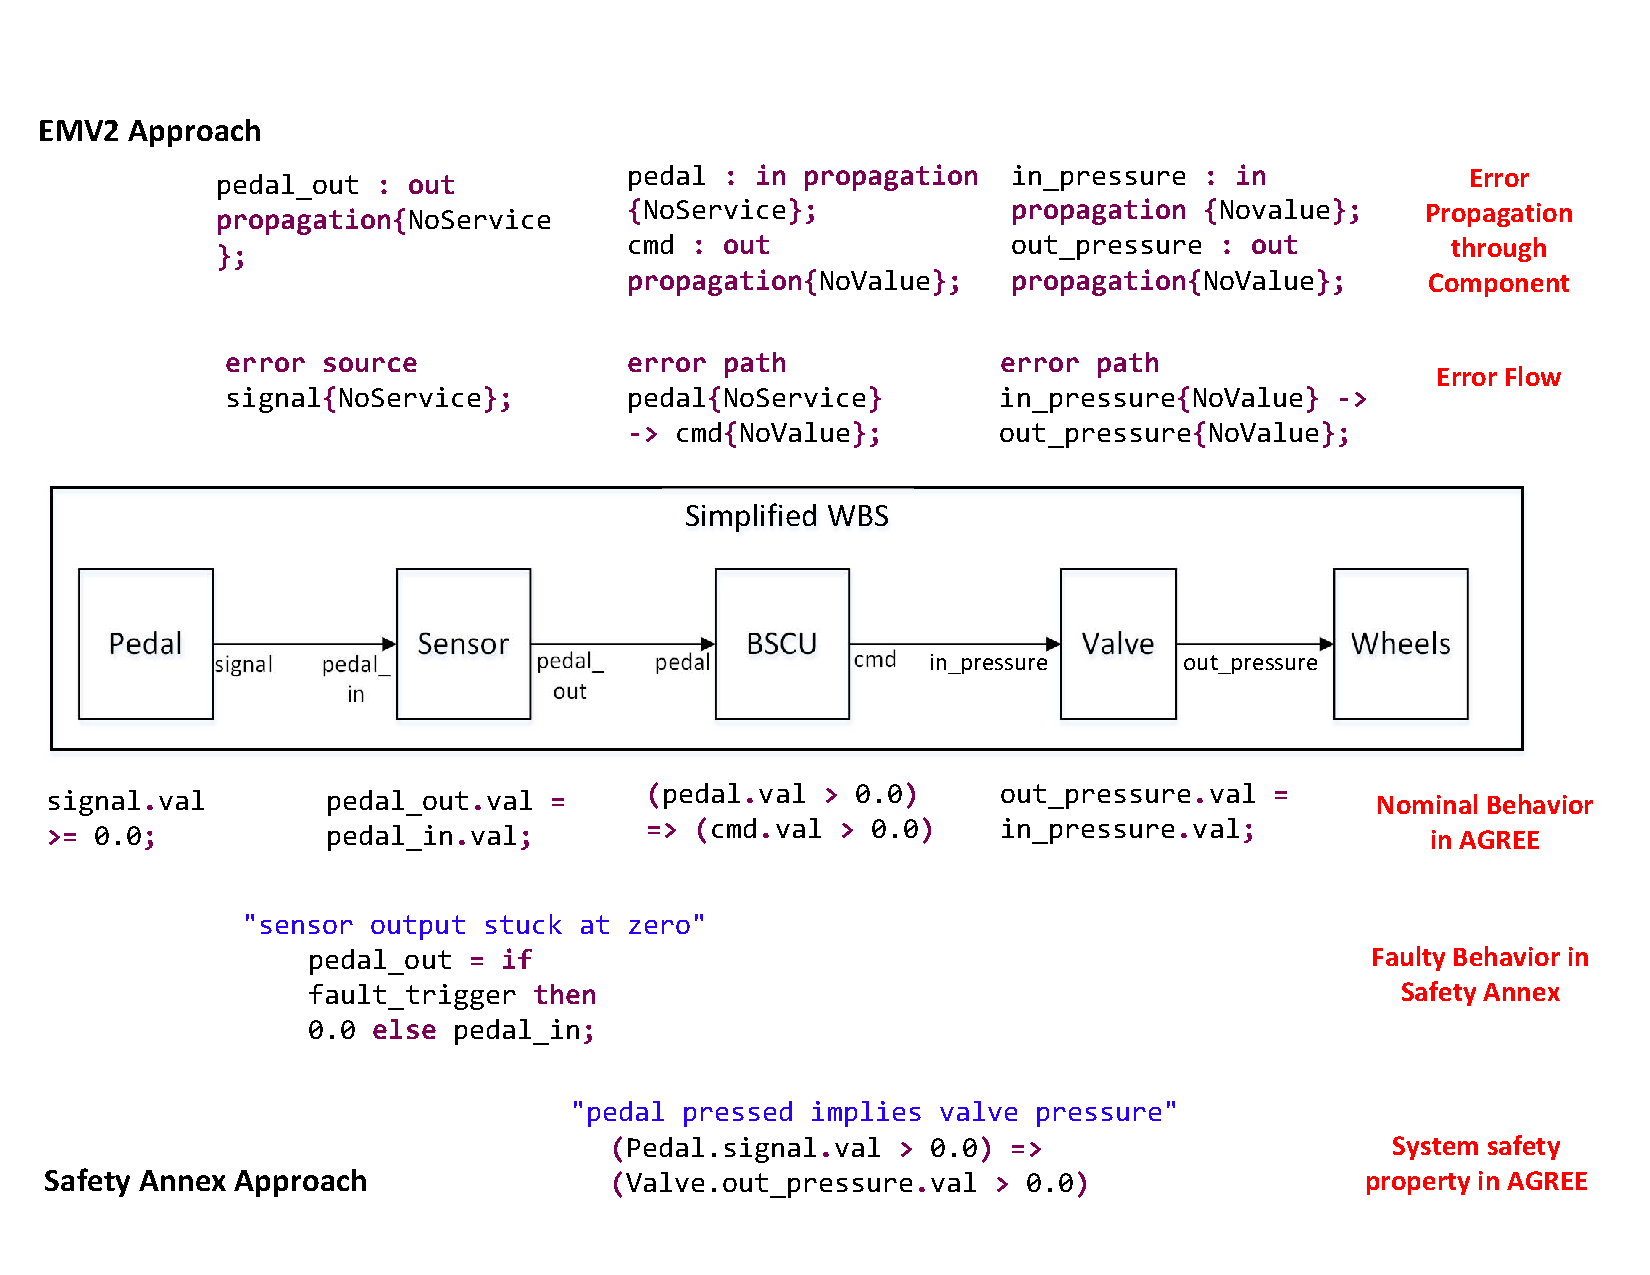
\includegraphics[trim=0 9 0 5,clip,width=\textwidth]{images/Comparison_with_EMV2.pdf}
	%\vspace{-0.3in}
	\caption{Differences between Safety Annex and EMV2}
	\label{fig:comparison_with_EMV2}
	%\vspace{-0.2in}
\end{figure} 

In this simplified WBS system, the physical signal from the Pedal component is detected by the Sensor and the pedal position value is passed to the Braking System Control Unit (BSCU) components.  The BSCU generates a pressure command to the Valve component which applies hydraulic brake pressure to the Wheels. 

In the EMV2 approach (top half of Figure~\ref{fig:comparison_with_EMV2}), the ``NoService'' fault is explicitly propagated through all of the components. These fault types are essentially tokens that do not capture any analyzable behavior. At the system level, analysis tools supporting the EMV2 annex can aggregate the propagation information from different components to compose an overall fault flow diagram or fault tree. 

When a fault is triggered in the Safety Annex (bottom half of Figure~\ref{fig:comparison_with_EMV2}), the output behavior of the Sensor component is modified. In this case the result is a ``stuck at zero'' error. The behavior of the BSCU receives a zero input and proceeds as if the pedal has not been pressed. This will cause the top level system contract to fail: {\em pedal pressed implies brake pressure output is positive}.
\end{comment}


\subsection{Explicit Propagation} 
Failures in hardware (HW) components can trigger behavioral faults in the system components that depend on them. For example, a CPU failure may trigger faulty behavior in the threads bound to that CPU. In addition, a failure in one HW component may trigger failure in other HW components located nearby, such as overheating, fire, or explosion
in the containment location. The safety annex provides the capability to explicitly model the impact of hardware failures on other faults, behavioral or non behavioral. 

To better model faults at the system level dependent on HW failures, a fault model element is introduced called a \textit{hardware fault}. Users are not required to specify behavioral effects for the HW faults, nor are data ports necessary on which to apply the fault definition. An example of a hardware fault declaration is shown in Figure~\ref{fig:hwFault} and describes a possible failure occurring between two co-located pumps. 
\begin{figure}[h!]
	%\vspace{-0.1in}
	\begin{center}
	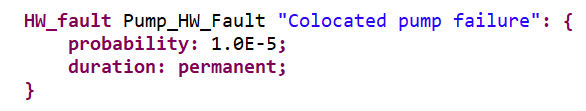
\includegraphics[width=.6\textwidth]{images/hw_fault2.png}
	\end{center}
	\vspace{-0.1in}
	\caption{Hardware Fault Definition}
	\label{fig:hwFault}
	%\vspace{-0.2in}
	%\vspace{-0.1in}
\end{figure}


Users specify dependencies between the HW component faults and faults that are defined in other components, either HW or SW. The hardware fault then acts as a trigger for dependent faults. This allows a simple propagation from the faulty HW component to the SW components that rely on it, affecting the behavior on the outputs of the affected SW components.

Assume that there exist a green and a blue hydraulic pump; these are located in the same compartment in the aircraft and an explosion in this compartment rendered both pumps inoperable. 
The HW fault definition can be modeled first in the green hydraulic pump component as shown in Figure~\ref{fig:hwFault}. The activation of this fault triggers the activation of related faults as seen in the \textit{propagate\_to} statement shown in Figure~\ref{fig:hwFaultProp}. 
Notice that these pumps need not be connected through a data port in order to specify this propagation. 

\begin{figure}[h!]
	%\vspace{-0.1in}
	\begin{center}
		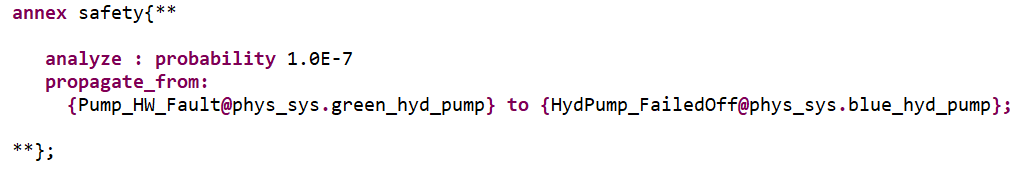
\includegraphics[width=1.0\textwidth]{images/hw_prop_stmt.png}
	\end{center}
	\vspace{-0.1in}
	\caption{Hardware Fault Propagation Statement}
	\label{fig:hwFaultProp}
	%\vspace{-0.2in}
	%\vspace{-0.1in}
\end{figure}

By allowing both kinds of error propagation, this allows great flexibility in modeling and allows an analyst to capture multiple kinds of faults. 


\section{Fault Hypothesis}
The fault hypothesis (also referred to as the fault analysis statement) resides in the AADL system implementation that is selected for verification. This may specify either a maximum number of faults that can be active at any point in execution:

\begin{figure}[h!]
	\vspace{-0.1in}
	%\begin{center}
		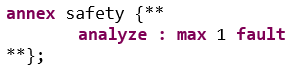
\includegraphics[width=0.4\textwidth]{images/hypothesisMaxN.png}
	%\end{center}
	\vspace{-0.1in}
	%%\caption{Max N Faults Analysis Statement}
	\label{fig:hypothesisMaxN}
\end{figure}
or that the only faults to be considered are those whose probability of simultaneous occurrence is above some probability threshold: 

\begin{figure}[h!]
	\vspace{-0.1in}
	%\begin{center}
		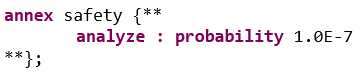
\includegraphics[width=0.5\textwidth]{images/hypothesisProb.png}
	%\end{center}
	\vspace{-0.1in}
	%\caption{Probability Analysis Statement}
	%\label{fig:hypothesisProb}
\end{figure}

Tying back to the fault tree analysis in traditional safety analysis, the former is analogous to restricting the cut sets to a specified maximum number of terms, and the latter is analogous to restricting the cut sets to only those whose probability is above some set value. In the former case, we assert that the sum of the true {\em fault\_\_trigger} variables is at or below some integer threshold.  In the latter, we determine all combinations of faults whose probabilities are above the specified probability threshold, and describe this as a proposition over {\em fault\_\_trigger} variables. 
%
With the introduction of dependent faults, active faults are divided into two categories: independently active (activated by its own triggering event) and dependently active (activated when the faults they depend on become active). The top level fault hypothesis applies to independently active faults. Faulty behaviors augment nominal behaviors whenever their corresponding faults are active (either independently active or dependently active).



\section{Asymmetric Fault Modeling}
\label{sec:byzantine}
A \textit{asymmetric} or \textit{Byzantine} fault is a fault that presents different symptoms to different observers~\cite{Driscoll-Byzantine-Fault}. In our modeling environment, asymmetric faults may be associated with a component that has a one-to-many ($1-n$) output to multiple ($n$) other components. In this configuration, a \textit{symmetric} fault will result in all destination components seeing the same faulty behavior from the source component. To capture the behavior of asymmetric faults (``different symptoms to different observers''), it was necessary to extend our fault modeling mechanism in AADL. A thorough description of the asymmetric modeling capability of the Safety Annex is shown in Chapter~\ref{chap:caseStudies} using a process ID example.

\subsection{Implementation of Asymmetric Faults}
To illustrate our implementation of asymmetric faults, assume a source component A has a 1-n output connected to four destination components (B-E) as shown in Figure~\ref{fig:commNodes} under ``Nominal System.'' If a symmetric fault was present on this output, all four connected components would see the same faulty behavior. An asymmetric fault should be able to present arbitrarily different values to the connected components. 

To this end, ``communication nodes'' are inserted on each connection from component A to components B, C, D, and E (shown in Figure~\ref{fig:commNodes} under ``Fault Model Architecture.'' From the users perspective, the asymmetric fault definition is associated with component A's output and the architecture of the model is unchanged from the nominal model architecture. Behind the scenes, these communication nodes are created to facilitate potentially different fault activations on each of these connections. The fault definition used on the output of component A will be inserted into each of these communication nodes as shown by the red circles at the communication node output in Figure~\ref{fig:commNodes}.
\begin{figure}[!htb]
        \center{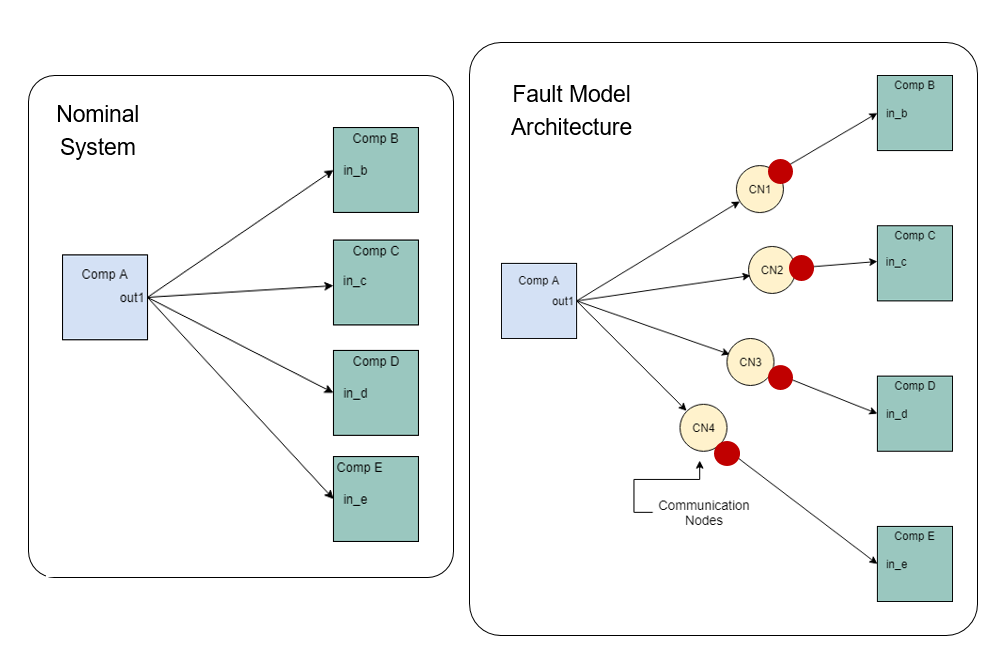
\includegraphics[width=\textwidth] {images/commNodes.png}}
        \caption{\label{fig:commNodes} Communication Nodes in Asymmetric Fault Implementation}
\end{figure}

\begin{figure}[!htb]
        \center{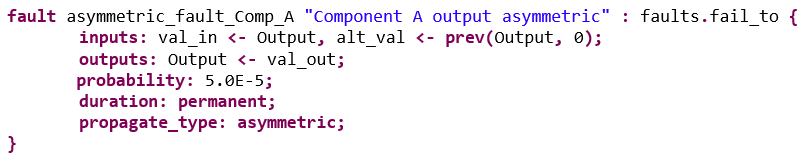
\includegraphics[width=\textwidth] {images/asymFaultDef.png}}
        \caption{\label{fig:asymFaultDef} Asymmetric Fault Definition in the Safety Annex}
\end{figure}

An asymmetric fault is defined for Component A as in Figure~\ref{fig:asymFaultDef}. This fault defines an asymmetric failure on Component A that when active, is stuck at a previous value (\textit{prev(Output, 0)}). This can be interpreted as the following: some connected components may only see the previous value of Comp A output and others may see the correct (current) value when the fault is active. This fault definition is injected into the communication nodes and which of the connected components see an incorrect value is completely nondeterministic. Any number of the communication node faults (0…all) may be active upon activation of the main asymmetric fault.

%\subsection{Referencing Fault Activation Status}
%To fully implement the agreement protocol, it must be possible to describe whether or not a subcomponent is failed by specifying if any faults defined for the subcomponents is activated. In the Safety Annex, this is made possible through the use of a \textit{fault activation} statement. Users can declare boolean \textit{eq} variables in the AGREE annex of the AADL system where the AGREE verification applies to that system's implementation. %in AGREE and in the implementations Safety Annex,  Users can then assign the activation status of specific faults to those \textit{eq} variables in Safety Annex of the AADL system implementation (the same place where the fault analysis statement resides).
%assigns this boolean \textit{eq} statement to a fault specific to a subcomponent.  This assignment links each specified AGREE boolean variable with the activation status of the specified fault activation literal. The AGREE boolean variable is true when and only when the fault is active. This additional feature of the Safety Annex allows users to state contracts of the form: if \texttt{sensor\_failed} then \texttt{do\_something}.

 


\section{Verification in the Presence of Faults}
\label{sec:analysisResults}
There are two main options for fault model analysis using the Safety Annex. The first option injects faults into the Lustre program based on the restrictions placed through the fault hypothesis. The Bounded Model Checker (BMC) engine used in JKind will find a {\em counterexample} to an invalid property. These counterexamples are returned to the user and include a trace of the system state that causes the violation. This includes any active faults that were part of that violation. The second option is used to generate minimal cut sets for the model. The details of minimal cut set generation can be found in Chapter~\ref{chap:mcsGen} and a full description of the analysis results for minimal cut set generation can be found there. 

\subsubsection{Counterexamples}
An important feature of a bounded temporal logic model checker is the ability to find counterexamples. When the model checker determines that a formula with a universal path quantifier (e.g., for all paths...) is false, it will find a computation path which demonstrates that the negation of the formula is true. Likewise when the model checker determines that an existential path quantifier is true (e.g., there exists a path...), it will find a computation path that demonstrates why the formula is true~\cite{clarke2018model}. 

The guarantees in an AGREE contract contain an implicit universal quantifier. Thus, if a guarantee states: $(a > b) \implies c$, this is translated as ``for all states, if $a > b$, then $c$." If this is invalid, the counterexample will include values within the constraints of the model for $a$, $b$, and $c$ such that $(a > b) \centernot \implies c$.

These counterexamples provide, in the nominal verification, insights into assumptions and guarantees for each component and how they may be strengthened to support correct behavior. In fault analysis, the counterexamples include active faults. Assuming that the nominal model (the model in the absence of faults) proves the specified properties, if verification in the presence of faults returns a counterexample, it is clear that an active fault caused the violation of the property. Insight into the state of the system when this occurs is invaluable to an analyst. This information can be used in the model-based safety assessment process to drive design changes. 

\subsubsection{Verification in the Presence of Faults: Max \textit{n} Analysis}
Using a max number of faults for the hypothesis, the user can constrain the number of simultaneously active faults in the model. The faults are added to the system subcomponents and a fault hypothesis statement is added to the component implementation. Given the constraint on the number of possible simultaneously active faults, the model checker attempts to prove the top level properties given these constraints. If this cannot be done, a counterexample is provided that shows which of the faults are active and which contracts are violated. We assume that the nominal model properties prove in the absence of faults.

The user can choose to perform either compositional or monolithic analysis using a max $n$ fault hypothesis. In compositional analysis, the analysis proceeds in a top down fashion. To prove the top level properties, the properties in the layer directly beneath the top level are used to perform the proof. The analysis proceeds in this manner. Users constrain the maximum number of faults within each layer of the model by specifying the maximum fault hypothesis statement to that layer. If any lower level property failed due to activation of faults, the property verification at the higher level can no longer be trusted because the higher level properties were proved based on the assumption that the direct sub-level contracts are valid. This form of analysis is helpful to see weaknesses in a given layer of the system. 

In monolithic analysis the layers of the model are flattened, which allows a direct correspondence between all faults in the model and their effects on the top level properties. As with compositional analysis, a counterexample shows these $n$ or less active faults. 

Returning to the PWR system example, we wish to see if the faults defined for the sensors contribute to a violation of the top level safety property (shut down occurs when and only when it should). The model has two distinct layers: top level with subsystems as subcomponents and leaf level with sensor subcomponents. If verification in the presence of faults is run compositionally with maximum 2 faults active, the results are as shown in Figure~\ref{fig:maxNPWRVerif}. 

\begin{figure}[h!]
	%\vspace{-0.1in}
	%\begin{center}
		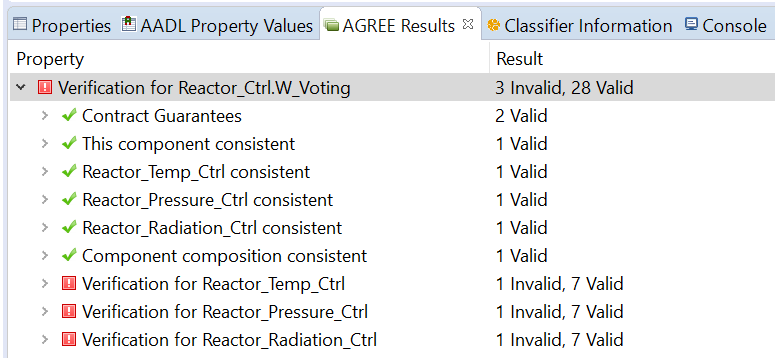
\includegraphics[width=0.8\textwidth]{images/maxNPWRVerif.png}
	%\end{center}
	%\vspace{-0.1in}
	\caption{PWR Verification with Maximum Two Faults Hypothesis}
	\label{fig:maxNPWRVerif}
\end{figure}

The top level verification passes because faults are not defined at that level. The leaf level verification, however, does not pass; the property at the subsystem level is violated. Selecting to view the counterexample, we see that two active faults on two sensors will violate the subsystem property. The counterexample spreadsheet view is shown in Figure~\ref{fig:maxNPWRVerifCoex}. 

\begin{figure}[h!]
	%\vspace{-0.1in}
	%\begin{center}
		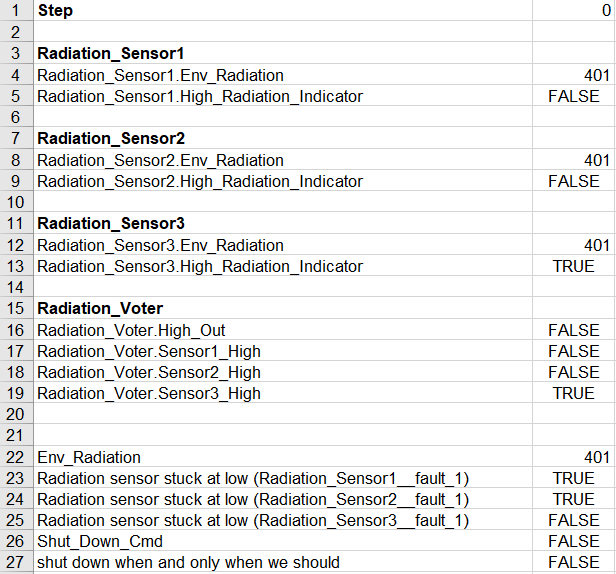
\includegraphics[width=0.6\textwidth]{images/maxNPWRVerifCoex.png}
	%\end{center}
	%\vspace{-0.1in}
	\caption{PWR Counterexample with Maximum Two-Faults Hypothesis}
	\label{fig:maxNPWRVerifCoex}
\end{figure}

A monolithic verification in the presence of faults will show that the top level safety property is violated; the subsystem guarantee directly supports the proof of the top level safety property. 

\subsubsection{Verification in the Presence of Faults: Probabilistic Analysis} 
Given a probabilistic fault hypothesis, this corresponds to performing analysis with the combinations of faults whose occurrence probability is less than the probability threshold. This is done by inserting assertions that allow those combinations in the Lustre code. If the model checker proves that the safety properties can be violated with any of those combinations, one of such combination will be shown in the counterexample. 

Probabilistic analysis done in this way must utilize the monolithic AGREE option. For compositional probabilistic analysis, see Chapter~\ref{chap:mcsGen} of this dissertation.

\begin{algorithm}[H]
	% \KwData{this text}
	% \KwResult{how to write algorithm with \LaTeX2e }
	$\mathcal{F} = \{\}$ : fault combinations above threshold \;
	$\mathcal{Q}$ : faults, $q_i$, arranged with probability high to low \;
	$\mathcal{R} = \mathcal{Q}$ , with $r \in \mathcal{R}$\;
	\While{$\mathcal{Q} \neq \{\} \land \mathcal{R} \neq \{\}$ }{
		$q =$ removeTopElement($\mathcal{Q}$) \;
		\For{$i=0:|\mathcal{R}|$}{
			$prob = q \times r_i$ \;
			\eIf{prob $<$ threshold}{
				removeTail($\mathcal{R}, j=i:|\mathcal{R}|$)\;
			}{
				add($\{q, r_i\}, \mathcal{Q}$)\;
				add($\{q, r_i\}, \mathcal{F}$)\;
			} % end if else
		} % end for
	} % end while
	\caption{Monolithic Probability Analysis}
	\label{alg:prob_monolithic}
\end{algorithm}

To perform this analysis, it is assumed that the non-hardware faults occur independently and possible combinations of faults are computed and passed to the Lustre model to be checked by the model checker. As seen in Algorithm 1, the computation first removes all faults from consideration that are too unlikely given the probability threshold. The remaining faults are arranged in a priority queue $\mathcal{Q}$ from high to low. Assuming independence in the set of faults, we take a fault with highest probability from the queue (step 5) and attempt to combine the remainder of the faults in $\mathcal{R}$ (step 7). If this combination is lower than the threshold (step 8), then we do not take into consideration this set of faults and instead remove the tail of the remaining faults in $\mathcal{R}$. 
 
In this calculation, we assume independence among the faults, but in the Safety Annex it is possible to define dependence between faults using a fault propagation statement. After fault combinations are computed using Algorithm~\ref{alg:prob_monolithic}, the triggered dependent HW faults are added to the combination as appropriate. 

In the PWR system, each sensor can fail with probability $1.0 \times 10^{-5}$ and the probabilistic threshold for the system safety property is given as $1.0 \times 10^{-9}$. Running monolithic verification in the presence of faults shows that given the voting mechanism, no faults will violate the safety property. By lowering the probabilistic threshold to $1.0 \times 10^{-10}$, the safety property is violated with two active faults on any sensor subsystem as shown in Figure~\ref{fig:probPWRVerif}.

\begin{figure}[h!]
	%\vspace{-0.1in}
	%\begin{center}
		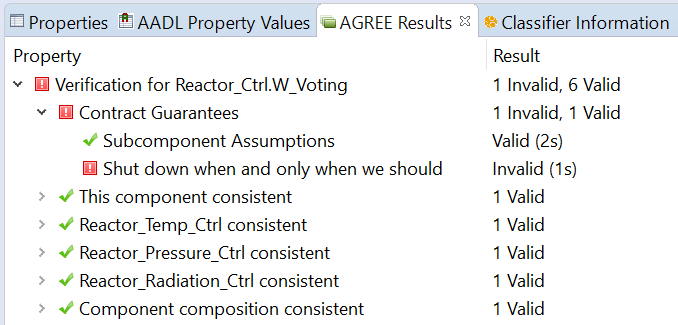
\includegraphics[width=0.8\textwidth]{images/probPWRVerif.png}
	%\end{center}
	%\vspace{-0.1in}
	\caption{PWR Verification with Probabilistic Hypothesis}
	\label{fig:probPWRVerif}
\end{figure}

Figure~\ref{fig:probPWRVerifCoex} shows a portion of the counterexample provided by the model checker for the probabilistic hypothesis of $1.0 \times 10^{-10}$. 

\begin{figure}[h!]
	%\vspace{-0.1in}
	%\begin{center}
		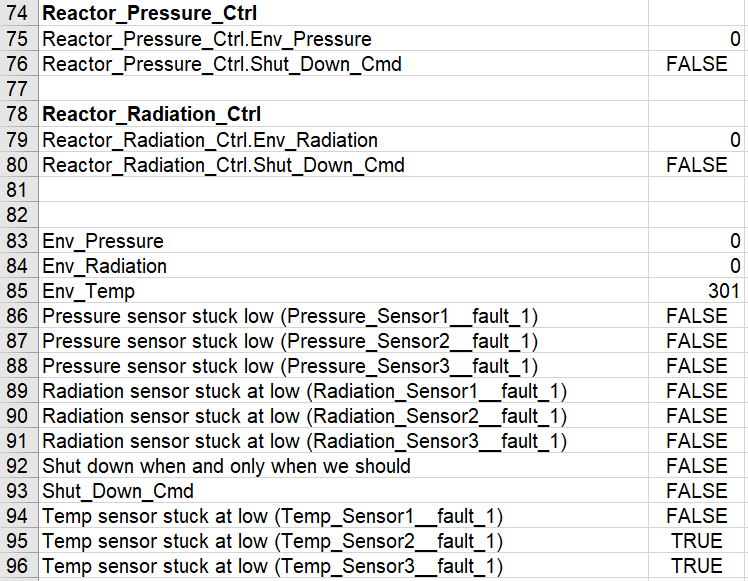
\includegraphics[width=0.6\textwidth]{images/probPWRVerifCoex.png}
	%\end{center}
	%\vspace{-0.1in}
	\caption{PWR Counterexample with Probabilistic Hypothesis}
	\label{fig:probPWRVerifCoex}
\end{figure}

The counterexample shows the active faults on the temperature subsystem: two faults are simultaneously active which violates the safety property. 

A benefit of utilizing the capabilities of counterexample generation is to ability for an analyst to view the dynamic behavior of a complex system and be able to understand the signal flow between behaviorally connected components. This aids in the design process when using model-based engineering methods and can greatly assist in design restructuring changes that may need to occur. It can be easy to see through counterexamples when a system is not resilient to a single fault, or when a combination of faults are sufficiently likely to occur together. Using these analysis capabilities support the objective to provide formal feedback to a safety engineer during the analysis of a complex critical system.

Up until this point, we have discussed modeling capabilities and counterexample generation using the safety annex for MBSA, but these counterexamples produce only a single path towards violation; in practice, safety analysts seek to find all minimal paths towards violation in terms of minimal cut sets. Given the analysis capabilities of a model checker in terms of proof cores -- the minimal set of model contracts required for a proof of the safety property -- we turn our attention towards leveraging this capability in terms of potentially active faults. 





